\chapter{Event Selection}
\label{chapter:event_selection}

This chapter defines the signal regions (SRs) targeting the processes shown in Figure~\ref{fig:u1_taunu_target_topologies}.
The analysis variables and preselection are introduced first, followed by the optimisation of the one-$b$-jet regions, the definition of the zero-$b$-jet regions, and a study of $\tau\tau$ signal contamination in the SRs.

\section{Preselection and variable definitions}
\label{sec:ch7_preselection}

\subsection{Analysis variables}
\label{subsec:ch7_variables}

The transverse mass $\mT$ of the $\tau$ and $\mpt$ system is defined as
    \begin{equation}
        \mT = \sqrt{2\pT^\tau\met\left[1-\cos\DphiTauMet\right]}.
        \label{eq:ch7_mt}
    \end{equation}
here $\DphiTauMet$ is the separation in $\phi$ between the $\tau$ momentum and $\mpt$.
The variable $\mT$ is used to probe the high-energy tail of the $\tau\nu$ final state, which is particularly sensitive to non-resonant leptoquark contributions~\cite{Endo2022NonResonant}.

The invariant masses $m_{b\tau}$ and $m_{j\tau}$ are defined as:
    \begin{equation}
        m_{b\tau}^{2} = (p_b+p_\tau)^2, \qquad m_{j\tau}^{2} = (p_{j_1}+p_\tau)^2,
        \label{eq:ch7_visible_masses}
    \end{equation}
    where $p_b$, $p_{j_1}$ and $p_\tau$ are four-momenta, and $j_1$ is the jet with the largest $\pT$, so-called the leading jet.
These two variables are used to probe the $b$-tagged and $b$-veto SRs, respectively.

\subsection{Multijet suppression and preselection}
\label{subsec:ch7_multijet}

Although the high $\met$ threshold rejects most multijet events, some can still enter the SRs and CRs due to the large multijet cross section. These events typically contain a misidentified $\tau$ and fake $\met$ due to the poor jet resolution. Therefore, further suppression is necessary.

Specifically, fake $\met$ is produced when an energetic jet is mismeasured. In this case, $\mpt$ points approximately towards that jet and it tends to be small compared with the $\pT$ of the mismeasured jet. On the other hand, in signal events, $\mpt$ from neutrinos has no such tendency.
Figure~\ref{fig:ch7_fake_met} illustrates this difference. The minimum jet--$\mpt$ separation in $\phi$ and the ratio $\metOverMinDphiJetPt$ are therefore used as discriminating variables. Here $\minDphiJetPt$ is the $\pT$ of the jet with the smallest $\DphiJetMet$.


\begin{figure}[htpb]
    \centering
    \begin{subfigure}{0.34\linewidth}
        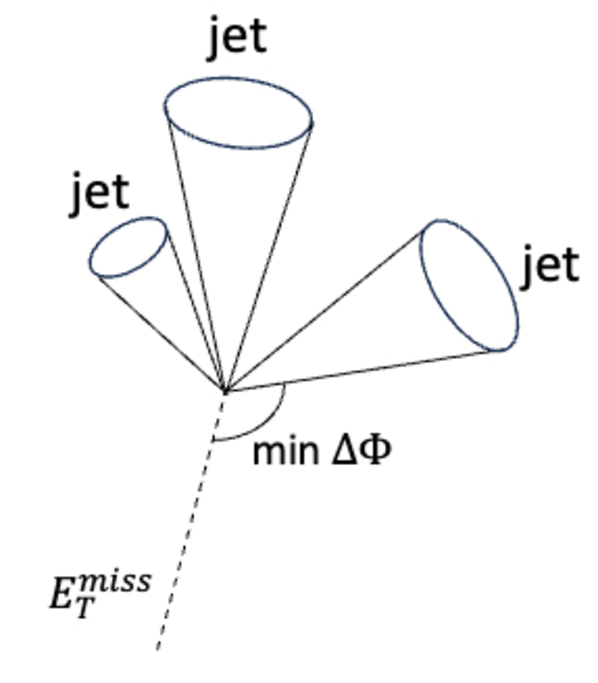
\includegraphics[width=\linewidth]{Figs/CH7/QCD/fake_met_signal.pdf}
        \caption{Signal.}
    \end{subfigure}\hspace{0.08\linewidth}
    \begin{subfigure}{0.34\linewidth}
        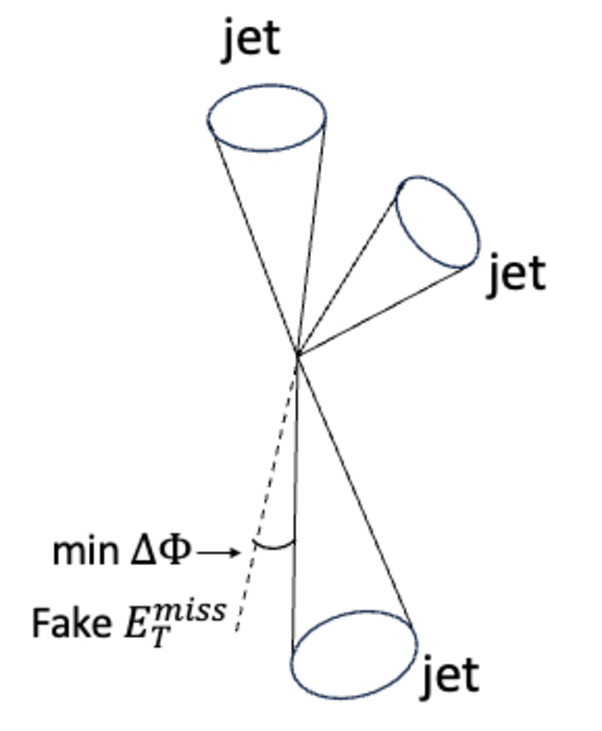
\includegraphics[width=\linewidth]{Figs/CH7/QCD/fake_met_multijets.pdf}
        \caption{Multijet background.}
    \end{subfigure}
    \caption[Missing momentum in signal and multijet events]{Schematic diagrams of (a) $\met$ from neutrinos in signal events and (b) fake $\met$ from a mismeasured energetic jet in multijet events.}
    \label{fig:ch7_fake_met}
\end{figure}

Events are retained if
\begin{equation}
    \minDphiJetMet>0.4 \quad\text{or}\quad \metOverMinDphiJetPt>6.
    \label{eq:ch7_qcd_cut}
\end{equation}
The study used to determine the thresholds above is presented in detail in Appendix~\ref{App:QCD_bkg_study}.

In addition to the multijet suppression requirement, the following preselection requirements are applied before the SR optimisation:
\begin{itemize}
  \item The lowest-threshold unprescaled $\met$ trigger to select events with large $\met$.
  \item $\met>200~\GeV$ for full trigger efficiency.
  \item Exactly one signal $\tau$.
  \item Signal electron/muon veto.
  \item Exactly one $b$-tagged jet for the one-$b$-jet SR ($\bTagSR$).
  \item At least one untagged jet and no $b$-tagged jets for the $b$-jet-veto SR ($\bVetoSR$).
\end{itemize}

\section[$\bTagSR$ optimisation and definition]{$\bTagSR$ optimisation and definition}
\label{sec:ch7_sr1b}

Event selection in $\bTagSR$ is optimised using a grid scan of thresholds on variables that help separate signal from background. $\bTagSR$-$\Res$ and $\bTagSR$-$\NonRes$ are optimised separately.

\subsection{Scan variables and criterion}
\label{subsec:ch7_scan}

$\pT^\tau$ and $\met$ are considered first, since energetic $\tau$ leptons and neutrinos are expected in the signal.
The $b$-jet $\pT$ is also used. An energetic $b$-jet from the leptoquark decay is expected in the resonant process, whereas the $b$-jet is typically softer in the non-resonant process. 
$\mT$ is used to distinguish non-resonant leptoquark exchange from the SM background.
A tighter $\mT$ threshold is therefore expected in $\bTagSR$-$\NonRes$ than in $\bTagSR$-$\Res$.
The invariant mass $m_{b\tau}$ is used to probe resonant $U_1\to b\tau$ decays.
$\DphiTauMet$ is used to select the back-to-back $\tau$ and $\mpt$ configuration of the non-resonant signal, which helps suppress the top-quark background.
On the other hand, in $\bTagSR$-$\Res$, small $\DphiTauMet$ values are favoured due to the high $\pT^b$ requirement.
The jet multiplicity is used to suppress $\ttbar$ events since they tend to have more jets than the signal events.
The thresholds used for the grid scan are summarised in Table~\ref{tab:ch7_scan_variables}.

\begin{table}[htbp]
    \centering
    \small
    \caption{Variable scan range for the $\bTagSR$ optimisation.}
    \label{tab:ch7_scan_variables}
    \begin{tabular}{lcc}
        \toprule
        Variable & $\bTagSR$-$\Res$ & $\bTagSR$-$\NonRes$ \\
        \midrule
        $\DphiTauMet$ & $<\{0.3,1.2,2.4,2.6,\pi\}$ & $>\{0.3,1.2,2.4,2.6\}$ \\
        $m_{b\tau}$ [$\GeV$] & $>\{0,800\}$ & N/A \\
        $\met$ [$\GeV$] & \multicolumn{2}{c}{$>\{200,250,300,350,400,500,600\}$} \\
        $\pT^\tau$ [$\GeV$] & \multicolumn{2}{c}{$>\{200,250,300,350,400,500,600\}$} \\
        $\mT$ [$\GeV$] & \multicolumn{2}{c}{$>\{100,200,300,400,500,600,700,800,900,1000\}$} \\
        $N_j-N_b$ & \multicolumn{2}{c}{$\leq\{1,2,3\}$} \\
        \bottomrule
    \end{tabular}
\end{table}

Note that only $m_{b\tau}>0$ and $800~\GeV$ are tested here. Since the signal mass resolution is only about 50\% and very few background events remain in the SRs, little improvement in sensitivity is expected from a finer mass threshold scan.

Different signal benchmarks are selected for the optimisations of each signal region. The optimisation for $\bTagSR$-$\Res$ uses $(\MU,\gU,\beta_L^{23})=(1.5~\TeV,1.5,0.6)$, where on-shell production is dominant.
For $\bTagSR$-$\NonRes$, the optimisation uses $(\MU,\gU,\beta_L^{23})=(2.5~\TeV,2.5,1.0)$, where $t$-channel exchange is dominant.
Interference is not included in the scan because its contribution is around $5$--$10\%$ in the parameter range probed by the $\bTagSR$ regions, as discussed in Appendix~\ref{app:signal_interference_study}. The selected cut combination is therefore not expected to change significantly when interference is included.

The expected sensitivity of each cut combination is evaluated using the significance $Z$, calculated as follows~\cite{ATL-PHYS-PUB-2020-025}:
\begin{equation}
    Z = \sqrt{2\left[n\ln\!\left(\frac{n(b+\sigma^2)}{b^2+n\sigma^2}\right)-\frac{b^2}{\sigma^2}\ln\!\left(\frac{b^2+n\sigma^2}{b(b+\sigma^2)}\right)\right]},
    \label{eq:ch7_optimisation_significance}
\end{equation}
where $s$ and $b$ are the expected signal and background event yields, $n=s+b$, and the background uncertainty is assumed to be $\sigma=0.3b$.

To obtain reliable results, the following two constraints are applied during the scan:
\begin{itemize}
    \item Cut combinations with $b\leq2$ are discarded.
    \item If a particular SM background (e.g. $\Wtaunu$) has a negative weighted yield, its contribution is set to zero.
\end{itemize}
The first constraint is applied to avoid zero background estimates caused by limited MC statistics. It also ensures reliable estimates of the minor backgrounds. As a result, the MC statistical uncertainties are limited to 31\% in the resonant SR and 40\% in the non-resonant SR.

An example of the significance scan is shown in Figure~\ref{fig:ch7_met_with_significance}, along with $N-1$ $\met$ distributions.\footnote{For a selection with $N$ requirements, an $N-1$ distribution is obtained by removing the requirement on the plotted variable while keeping the other $N-1$ requirements. Here, the $\met$ requirement is removed.}
For each bin in the lower significance panels, $Z$ is calculated using the signal and background yields summed above the corresponding threshold. Points with $b\leq2$ are excluded from the cut choice.
The largest $Z$ is therefore obtained at $200~\GeV$ for $\bTagSR$-$\Res$ and $400~\GeV$ for $\bTagSR$-$\NonRes$. A similar procedure is applied to the other variables.

% \begin{figure}[htbp]
%     \centering
%     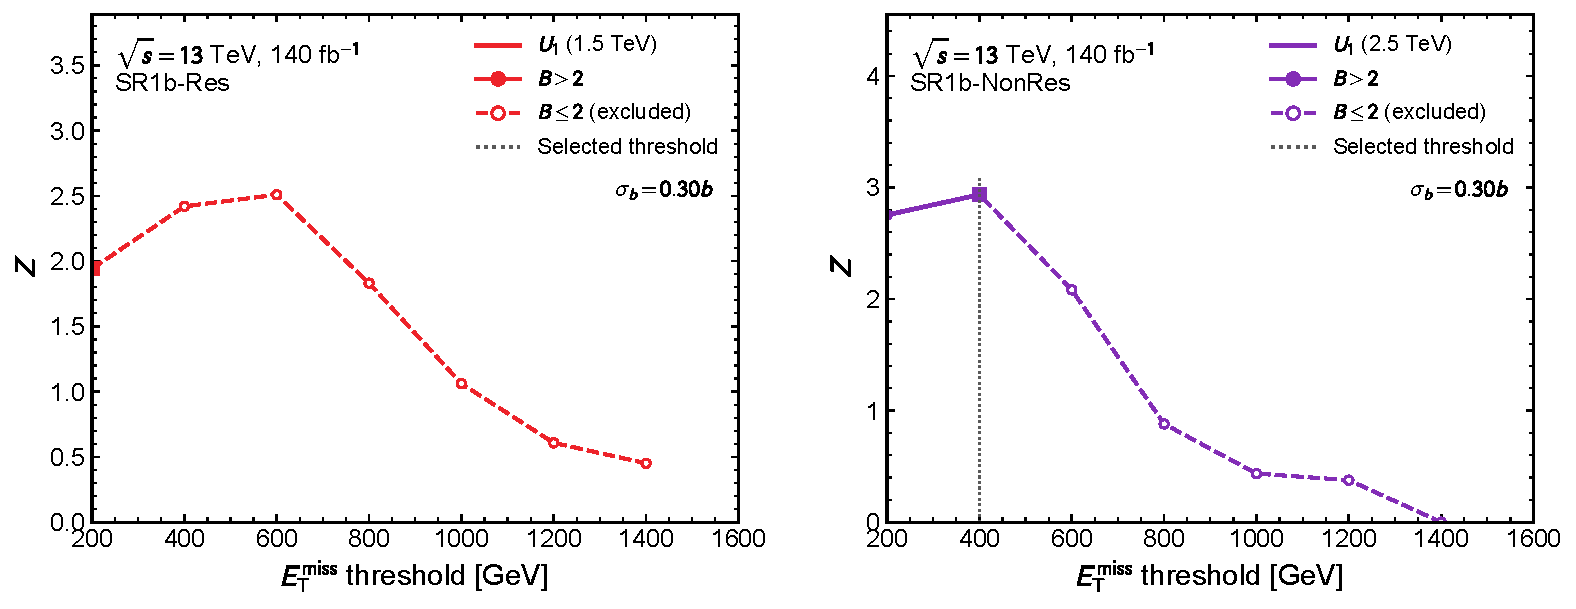
\includegraphics[width=\linewidth]{Figs/CH7/significance/SR1b_met_significance_scan.pdf}
%     \caption[SR1b significance scan in missing transverse momentum]{Approximate significance as a function of the $\met$ threshold for $\bTagSR$-$\Res$ (left) and $\bTagSR$-$\NonRes$ (right), using the pure BSM benchmarks $(\MU,\gU,\beta_L^{23})=(1.5~\TeV,1.5,0.6)$ and $(2.5~\TeV,2.5,1.0)$, respectively. The $N-1$ distributions are integrated above each threshold and Eq.~\ref{eq:ch7_optimisation_significance} is evaluated with $\sigma=0.30b$. Open markers and dashed segments indicate points with $b\leq2$, which are excluded from the cut choice. The selected thresholds are marked by squares and vertical dotted lines.}
%     \label{fig:ch7_met_significance_scan}
% \end{figure}

\begin{figure}[htpb]
    \centering
    \begin{subfigure}{0.8\linewidth}
        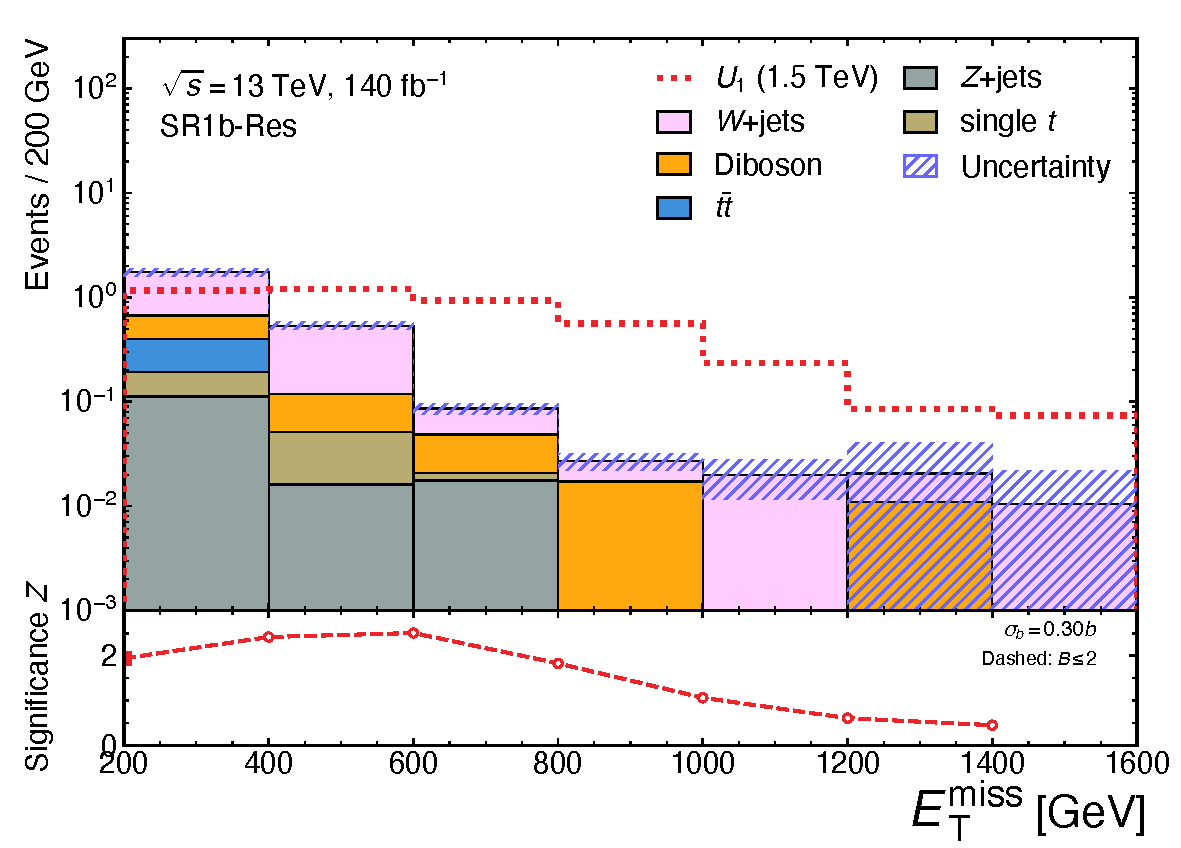
\includegraphics[width=\linewidth]{Figs/CH7/significance/SR1b_Res_met_with_significance.pdf}
        \caption{$\bTagSR$-$\Res$.}
    \end{subfigure}\\[0.5em]
    \begin{subfigure}{0.8\linewidth}
        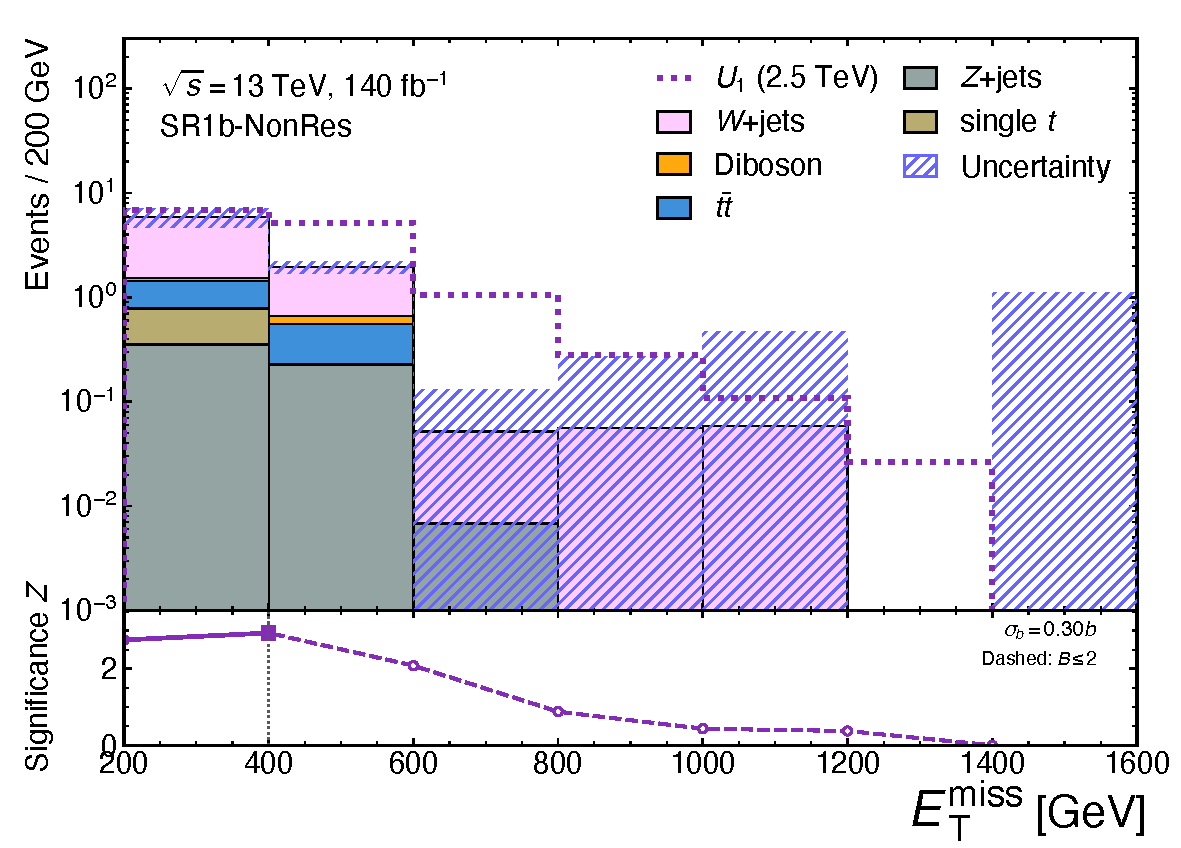
\includegraphics[width=\linewidth]{Figs/CH7/significance/SR1b_NonRes_met_with_significance.pdf}
        \caption{$\bTagSR$-$\NonRes$.}
    \end{subfigure}
    \caption[SR1b missing transverse momentum with significance $Z$]{$N-1$ $\met$ distributions and the corresponding significance $Z$. $Z$ is calculated from the signal and background yields above each threshold, with $\sigma=0.30b$. Dashed segments of the $Z$ curves indicate regions where $b\leq2$.}
    \label{fig:ch7_met_with_significance}
\end{figure}

\clearpage
\subsection[SR1b-Res definition]{$\bTagSR$-$\Res$}
\label{subsec:ch7_sr1b_res}

The definition and cutflow for $\bTagSR$-$\Res$ are summarised in Table~\ref{tab:ch7_cutflow_res}, using the resonant optimisation benchmark $(\MU,\gU,\beta_L^{23})=(1.5~\TeV,1.5,0.6)$.
A single event count with $m_{b\tau}>800~\GeV$ is used because the simulated background statistics at high $m_{b\tau}$ are insufficient for a fit to the mass distribution.

\begin{table}[htbp]
    \centering
    \small
    \caption{Signal and background cutflow for $\bTagSR$-$\Res$. The signal is evaluated at $(\MU,\gU,\beta_L^{23})=(1.5~\TeV,1.5,0.6)$. The uncertainties are from MC statistics only.}
    \label{tab:ch7_cutflow_res}
    \setlength{\tabcolsep}{3pt}
    \resizebox{\linewidth}{!}{%
    \begin{tabular}{lrrrrrrr}
        \toprule
        Requirement & Signal & $\ttbar$ & Single top & $W$+jets & $Z$+jets & Diboson & Total background \\
        \midrule
        Baseline & $35.2\pm0.4$ & $1043.0\pm6.9$ & $283.8\pm3.4$ & $2156.9\pm16.1$ & $369.2\pm7.7$ & $173.9\pm2.7$ & $4027.3\pm19.7$ \\
        $\pT^\tau>200~\GeV$ & $19.9\pm0.3$ & $32.3\pm1.3$ & $11.8\pm0.5$ & $108.9\pm9.4$ & $30.4\pm4.7$ & $9.7\pm0.6$ & $193.1\pm10.6$ \\
        $\met>200~\GeV$ & $19.9\pm0.3$ & $32.3\pm1.3$ & $11.8\pm0.5$ & $108.9\pm9.4$ & $30.4\pm4.7$ & $9.7\pm0.6$ & $193.1\pm10.6$ \\
        $\mT>200~\GeV$ & $19.4\pm0.3$ & $25.1\pm1.1$ & $9.2\pm0.4$ & $79.2\pm9.4$ & $24.2\pm4.7$ & $6.9\pm0.5$ & $143.6\pm10.6$ \\
        $m_{b\tau}>800~\GeV$ & $4.9\pm0.1$ & $0.4\pm0.2$ & $0.4\pm0.1$ & $2.8\pm0.4$ & $1.1\pm0.2$ & $0.5\pm0.1$ & $5.2\pm0.5$ \\
        $N_j-N_b\leq3$ & $4.7\pm0.1$ & $0.3\pm0.1$ & $0.2\pm0.1$ & $2.5\pm0.4$ & $0.9\pm0.2$ & $0.4\pm0.1$ & $4.3\pm0.5$ \\
        $\pT^b>250~\GeV$ & $4.2\pm0.1$ & $0.2\pm0.1$ & $0.1\pm0.1$ & $1.5\pm0.2$ & $0.2\pm0.1$ & $0.4\pm0.1$ & $2.4\pm0.3$ \\
        \bottomrule
    \end{tabular}
    }
\end{table}

As a result, the expected signal and background yields are 4.2 and 2.4 events, respectively, giving $Z=1.95$.

The background is dominated by $W(\to\tau\nu)$+jets, which contributes approximately $64\%$.
Approximately $16\%$ is contributed by diboson production.
The top-quark contribution consists of $\ttbar$ ($8\%$) and single-top production ($5\%$), with the latter mainly from the $Wt$ process.
These events are mainly from $\ttbar\to b\tau\nu\,\bar b\tau\nu$ or $Wt\to b\tau\nu\,\tau\nu$ when only one $\tau$ is selected and the other is misidentified as a jet.
A smaller contribution is provided by $Z(\to\tau\tau)$+jets, while the $Z(\to\nu\nu)$+jets contribution is negligibly small.

The $N-1$ distributions in $\bTagSR$-$\Res$ with relaxed kinematic requirements are shown in Figure~\ref{fig:ch7_sr1b_res_distributions}.
To reduce statistical fluctuations, the thresholds on the correlated variables $\mT$ and $\pT^\tau$ are both lowered to $100~\GeV$.

For the $1.5~\TeV$ benchmark, the $m_{b\tau}$ peak is shifted to about $900~\GeV$ because the neutrino from the $\tau$ decay is not included in the reconstructed mass.
The mass distribution is also broadened by the missing neutrino momentum and poor jet reconstruction resolution.

\begin{figure}[htpb]
    \centering
    \begin{subfigure}{0.48\linewidth}
        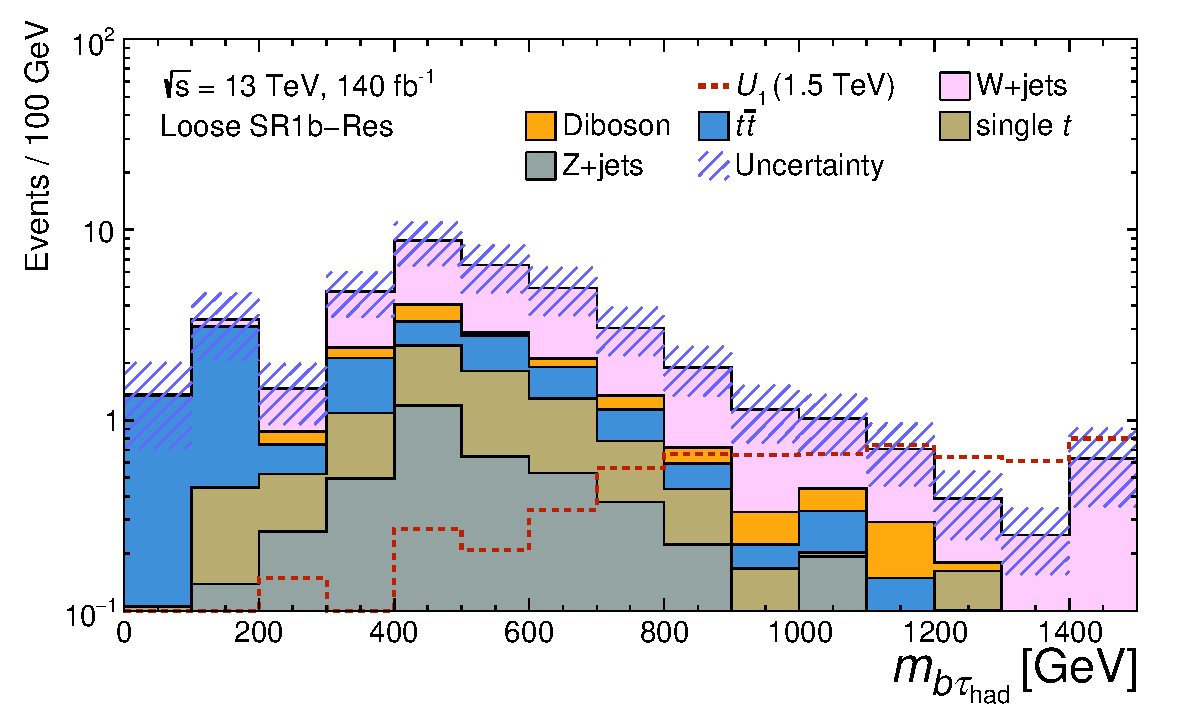
\includegraphics[width=\linewidth]{Figs/CH7/SR1b_Res_InvM.pdf}
        \caption{$m_{b\tau_{\mathrm{had}}}$.}
    \end{subfigure}\hfill
    \begin{subfigure}{0.48\linewidth}
        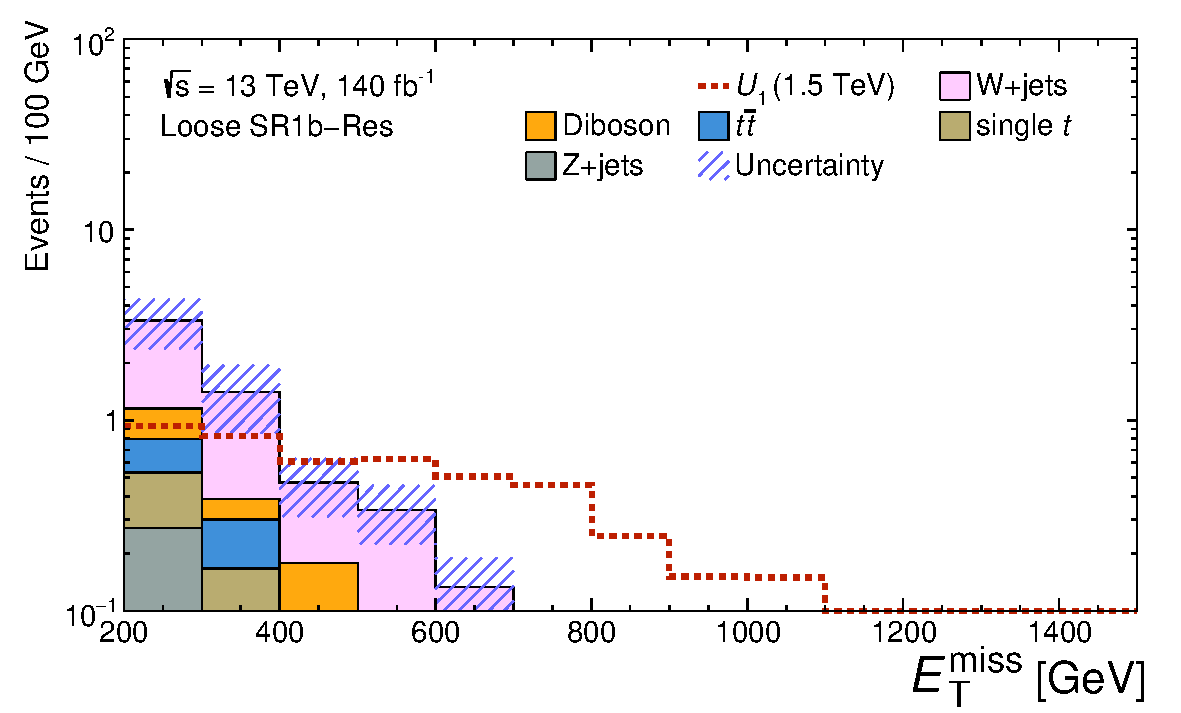
\includegraphics[width=\linewidth]{Figs/CH7/SR1b_Res_met.pdf}
        \caption{$\met$.}
    \end{subfigure}\\
    \begin{subfigure}{0.48\linewidth}
        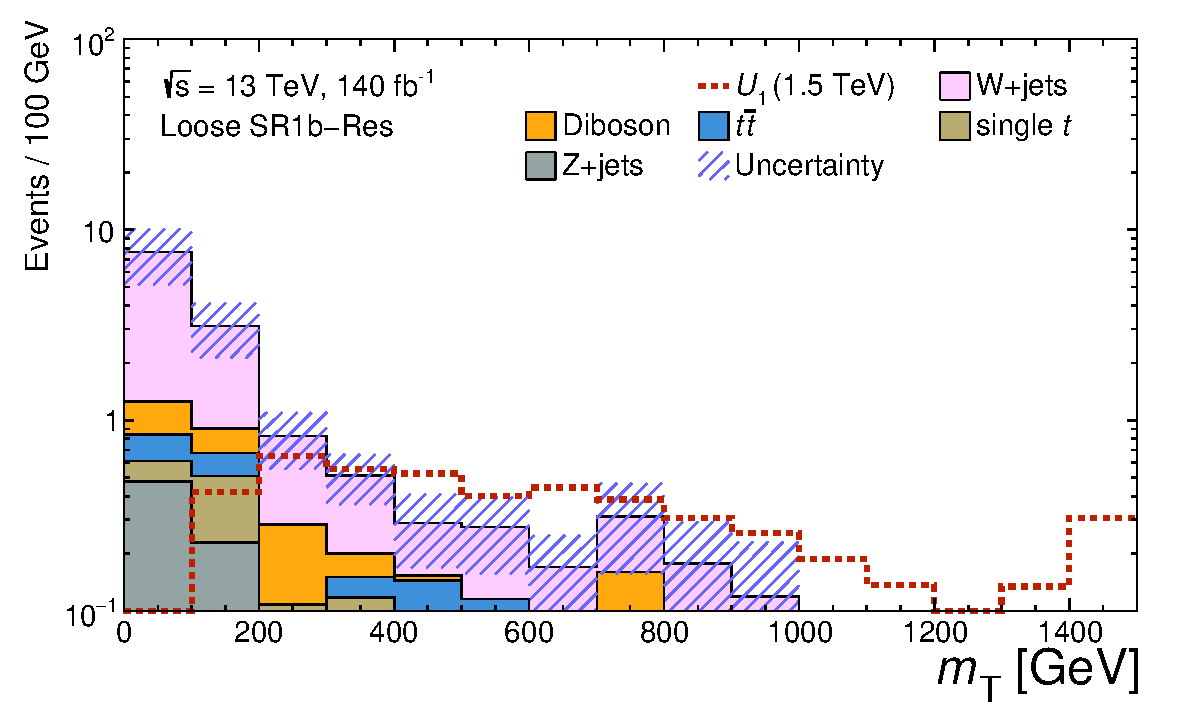
\includegraphics[width=\linewidth]{Figs/CH7/SR1b_Res_mT.pdf}
        \caption{$\mT$.}
    \end{subfigure}\hfill
    \begin{subfigure}{0.48\linewidth}
        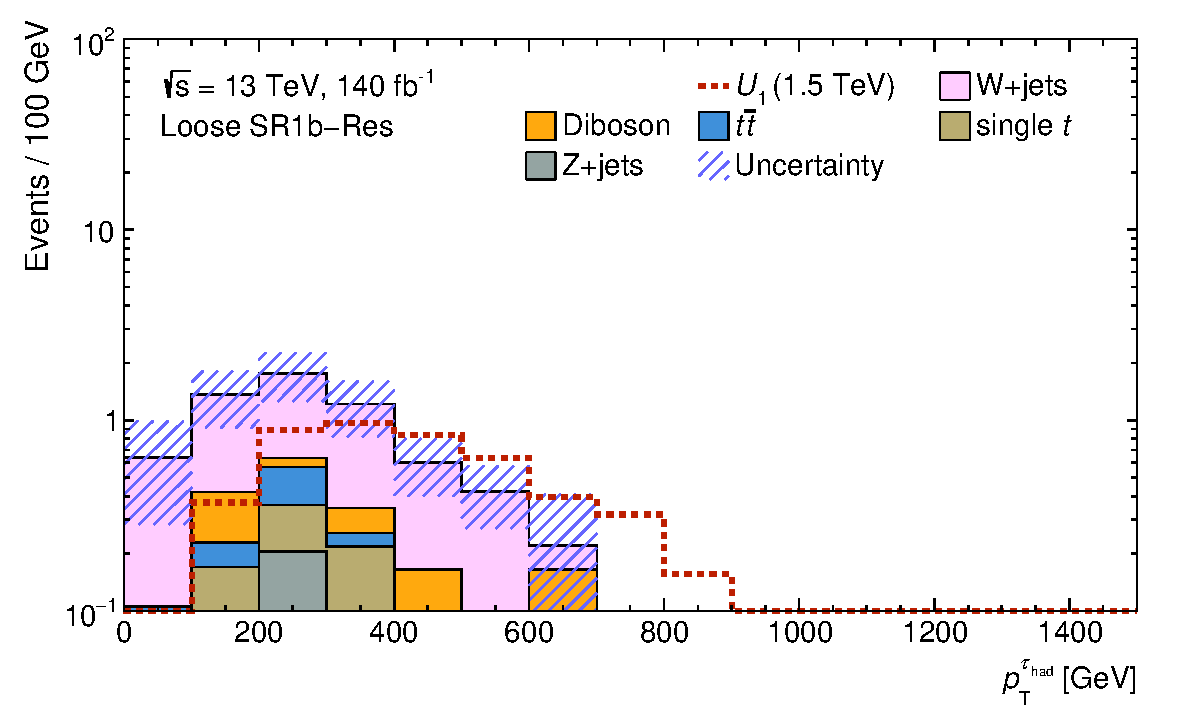
\includegraphics[width=\linewidth]{Figs/CH7/SR1b_Res_tau_pT.pdf}
        \caption{$\pT^{\tau_{\mathrm{had}}}$.}
    \end{subfigure}\\
    \begin{subfigure}{0.48\linewidth}
        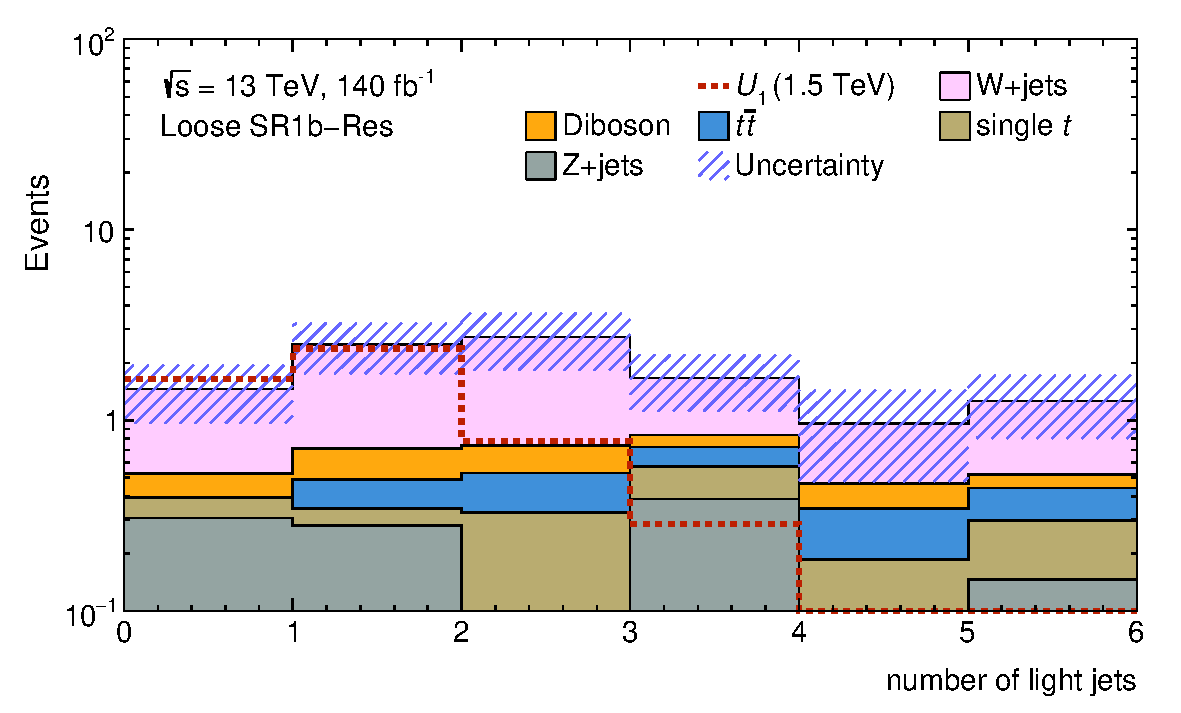
\includegraphics[width=\linewidth]{Figs/CH7/SR1b_Res_nlightjets.pdf}
        \caption{Number of light jets.}
    \end{subfigure}\hfill
    \begin{subfigure}{0.48\linewidth}
        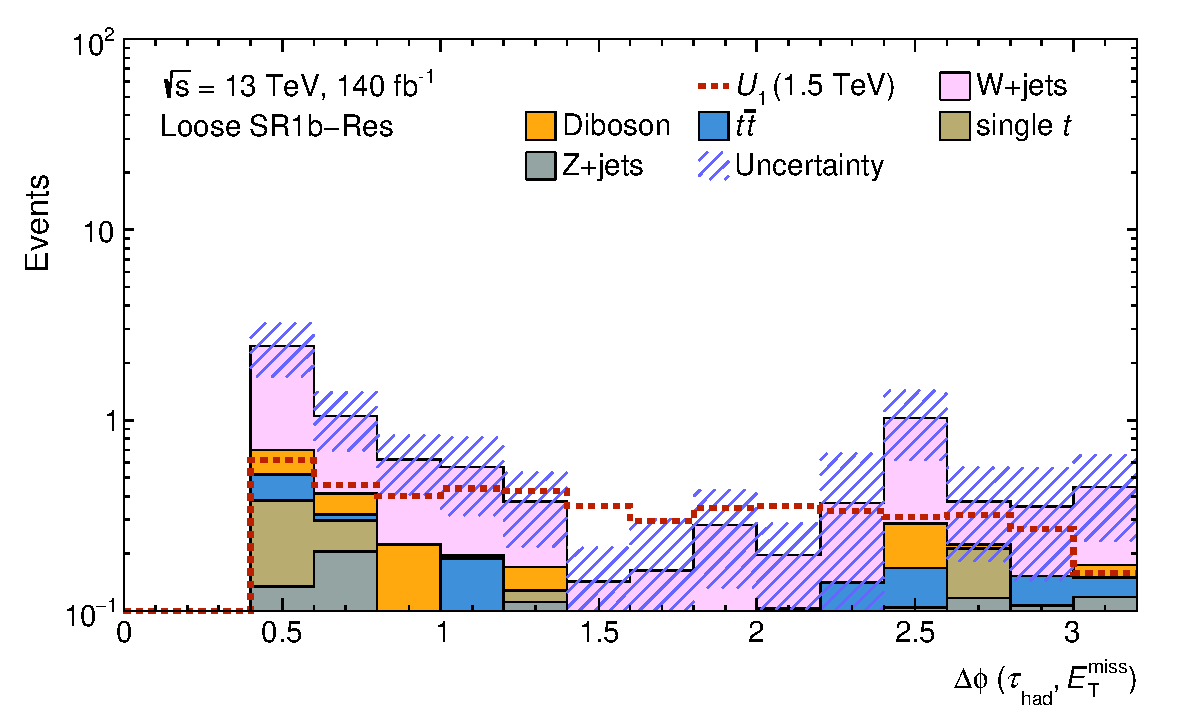
\includegraphics[width=\linewidth]{Figs/CH7/SR1b_Res_dphi.pdf}
        \caption{$\Delta\phi(\tau_{\mathrm{had}},\met)$.}
    \end{subfigure}
    \caption[Loose N-1 distributions in SR1b-Res]{$N-1$ distributions in the loose $\bTagSR$-$\Res$ region. The $\mT$ and $\pT^{\tau_{\mathrm{had}}}$ thresholds are reduced to $100~\GeV$. The red dashed line represents the signal at $(\MU,\gU,\beta_L^{23})=(1.5~\TeV,1.5,0.6)$. Systematic uncertainties are also included. The red arrows indicate the final selection thresholds.}
    \label{fig:ch7_sr1b_res_distributions}
\end{figure}

\clearpage
\subsection[SR1b-NonRes definition]{$\bTagSR$-$\NonRes$}
\label{subsec:ch7_sr1b_nonres}

The definition and cutflow for $\bTagSR$-$\NonRes$ are summarised in Table~\ref{tab:ch7_cutflow_nonres}, using the non-resonant benchmark $(\MU,\gU,\beta_L^{23})=(2.5~\TeV,2.5,1.0)$.
No $m_{b\tau}$ requirement is applied in the optimisation because the $b$-jet and $\tau$ do not reconstruct an on-shell leptoquark in the target topology.
A single event count is also used in this region.

\begin{table}[htbp]
    \centering
    \small
    \caption{Signal and background cutflow for $\bTagSR$-$\NonRes$. The signal is evaluated at $(\MU,\gU,\beta_L^{23})=(2.5~\TeV,2.5,1.0)$. The uncertainties are from MC statistics only.}
    \label{tab:ch7_cutflow_nonres}
    \setlength{\tabcolsep}{3pt}
    \resizebox{\linewidth}{!}{%
    \begin{tabular}{lrrrrrrr}
        \toprule
        Requirement & Signal & $\ttbar$ & Single top & $W$+jets & $Z$+jets & Diboson & Total background \\
        \midrule
        Baseline & $111.0\pm4.2$ & $1043.0\pm6.9$ & $283.8\pm3.4$ & $2156.9\pm16.1$ & $369.2\pm7.7$ & $173.9\pm2.7$ & $4027.3\pm19.7$ \\
        $\pT^\tau>200~\GeV$ & $70.5\pm3.8$ & $32.3\pm1.3$ & $11.8\pm0.5$ & $108.9\pm9.4$ & $30.4\pm4.7$ & $9.7\pm0.6$ & $193.1\pm10.7$ \\
        $\met>400~\GeV$ & $26.4\pm2.3$ & $2.1\pm0.3$ & $0.8\pm0.1$ & $9.0\pm1.5$ & $1.4\pm0.3$ & $1.8\pm0.2$ & $15.1\pm1.6$ \\
        $\mT>600~\GeV$ & $24.0\pm2.2$ & $0.7\pm0.2$ & $0.3\pm0.1$ & $3.9\pm1.5$ & $0.8\pm0.2$ & $0.7\pm0.2$ & $6.4\pm1.6$ \\
        $\DphiTauMet>1.2$ & $23.8\pm2.2$ & $0.7\pm0.2$ & $0.3\pm0.1$ & $3.8\pm1.5$ & $0.8\pm0.2$ & $0.7\pm0.2$ & $6.4\pm1.6$ \\
        $N_j-N_b\leq1$ & $17.2\pm2.1$ & $0.3\pm0.1$ & $0.1\pm0.1$ & $1.6\pm1.4$ & $0.4\pm0.1$ & $0.4\pm0.2$ & $2.8\pm1.4$ \\
        $50<\pT^b<250~\GeV$ & $6.6\pm0.7$ & $0.3\pm0.1$ & $0.0\pm0.1$ & $1.6\pm0.5$ & $0.2\pm0.1$ & $0.1\pm0.1$ & $2.1\pm0.5$ \\
        \bottomrule
    \end{tabular}
    }
\end{table}

As a result, the expected signal and background yields are 6.6 and 2.1 events, respectively, giving $Z=2.94$.

The background is also dominated by $W(\to\tau\nu)$+jets, which contributes approximately $69\%$.
Approximately $16\%$ is contributed by $\ttbar$, followed by $Z(\to\tau\tau)$+jets ($8\%$) and diboson production ($5\%$).
The $Z(\to\tau\tau)$+jets events pass the selection when only one $\tau$ is selected, with $\met$ from the $\tau$ neutrinos.
$Z(\to\nu\nu)$+jets is still the main source of fake $\tau$ background.
Multijet production is negligible after the cleaning and full SR requirements.

The yields and significances for both regions are summarised in Table~\ref{tab:ch7_prefit_yields}.

\begin{table}[htbp]
    \centering
    \small
    \caption{Signal and background yields for the two optimisation benchmarks in the final $\bTagSR$ selections. The approximate significance is evaluated with $\sigma=0.30b$.}
    \label{tab:ch7_prefit_yields}
    \begin{tabular}{lcrrr}
        \toprule
        SR & $(\MU,\gU,\beta_L^{23})$ & $S$ & $B$ & $Z$ \\
        \midrule
        $\bTagSR$-$\Res$ & $(1.5~\TeV,1.5,0.6)$ & 4.262 & 2.439 & 1.95 \\
        $\bTagSR$-$\NonRes$ & $(2.5~\TeV,2.5,1.0)$ & 6.583 & 2.097 & 2.94 \\
        \bottomrule
    \end{tabular}
\end{table}

The $N-1$ distributions in $\bTagSR$-$\NonRes$ with relaxed kinematic requirements are shown in Figure~\ref{fig:ch7_sr1b_nonres_distributions}.
To reduce statistical fluctuations, the $\mT$, $\met$ and $\pT^\tau$ thresholds are each lowered by $100~\GeV$, while the baseline requirement $\met>200~\GeV$ is retained.

\begin{figure}[htpb]
    \centering
    \begin{subfigure}{0.48\linewidth}
        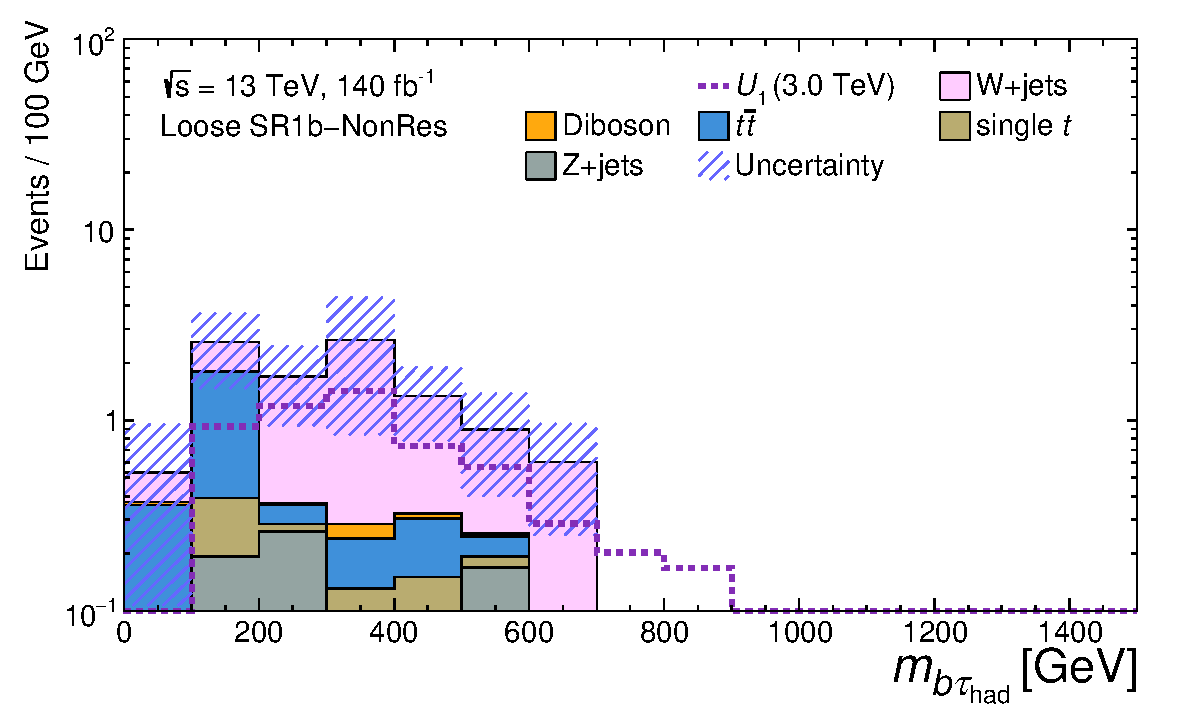
\includegraphics[width=\linewidth]{Figs/CH7/SR1b_NonRes_InvM.pdf}
        \caption{$m_{b\tau_{\mathrm{had}}}$.}
    \end{subfigure}\hfill
    \begin{subfigure}{0.48\linewidth}
        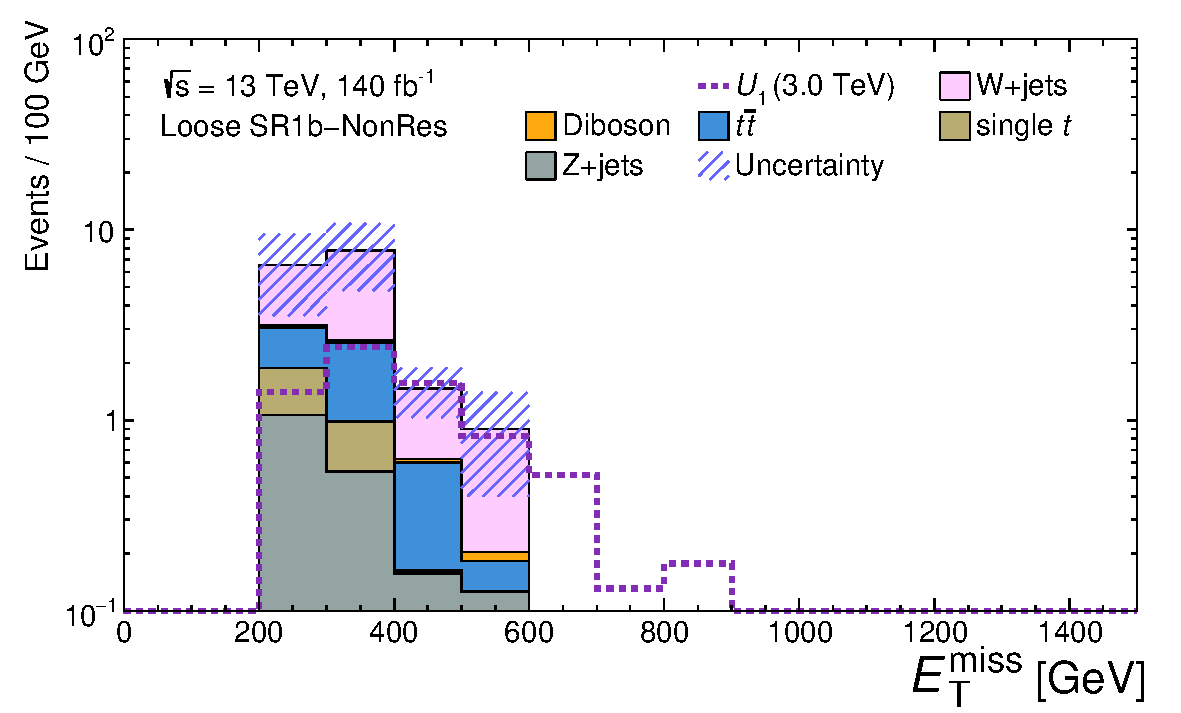
\includegraphics[width=\linewidth]{Figs/CH7/SR1b_NonRes_met.pdf}
        \caption{$\met$.}
    \end{subfigure}\\
    \begin{subfigure}{0.48\linewidth}
        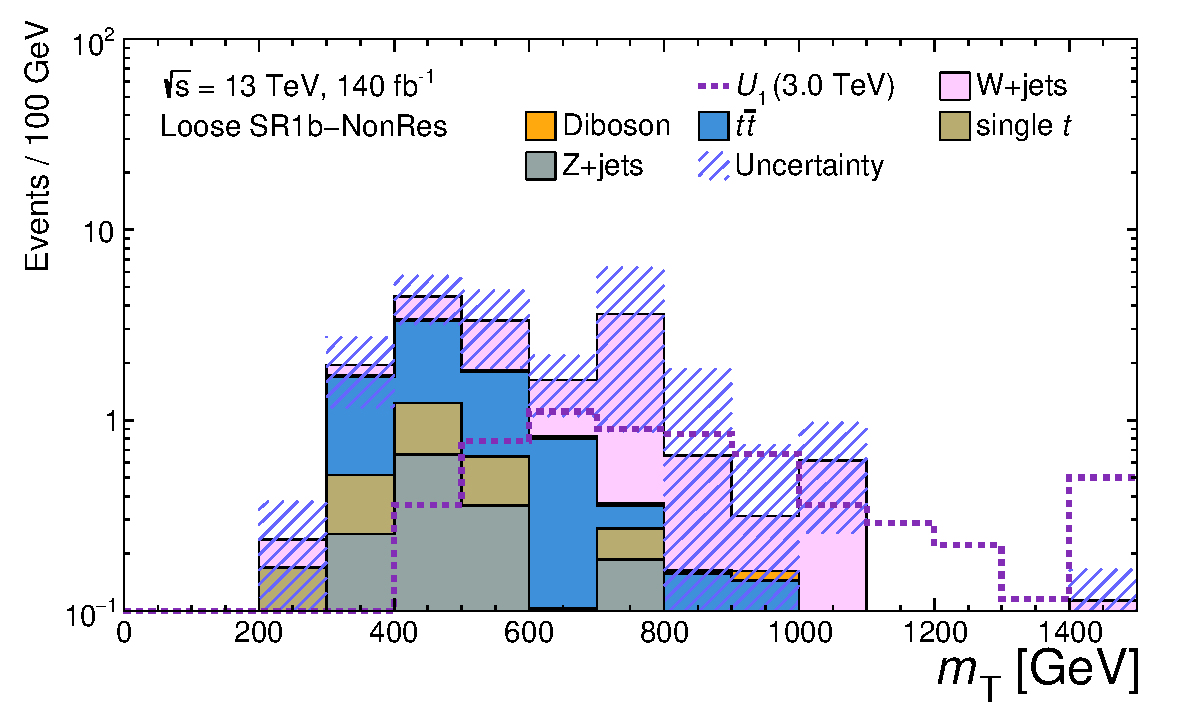
\includegraphics[width=\linewidth]{Figs/CH7/SR1b_NonRes_mT.pdf}
        \caption{$\mT$.}
    \end{subfigure}\hfill
    \begin{subfigure}{0.48\linewidth}
        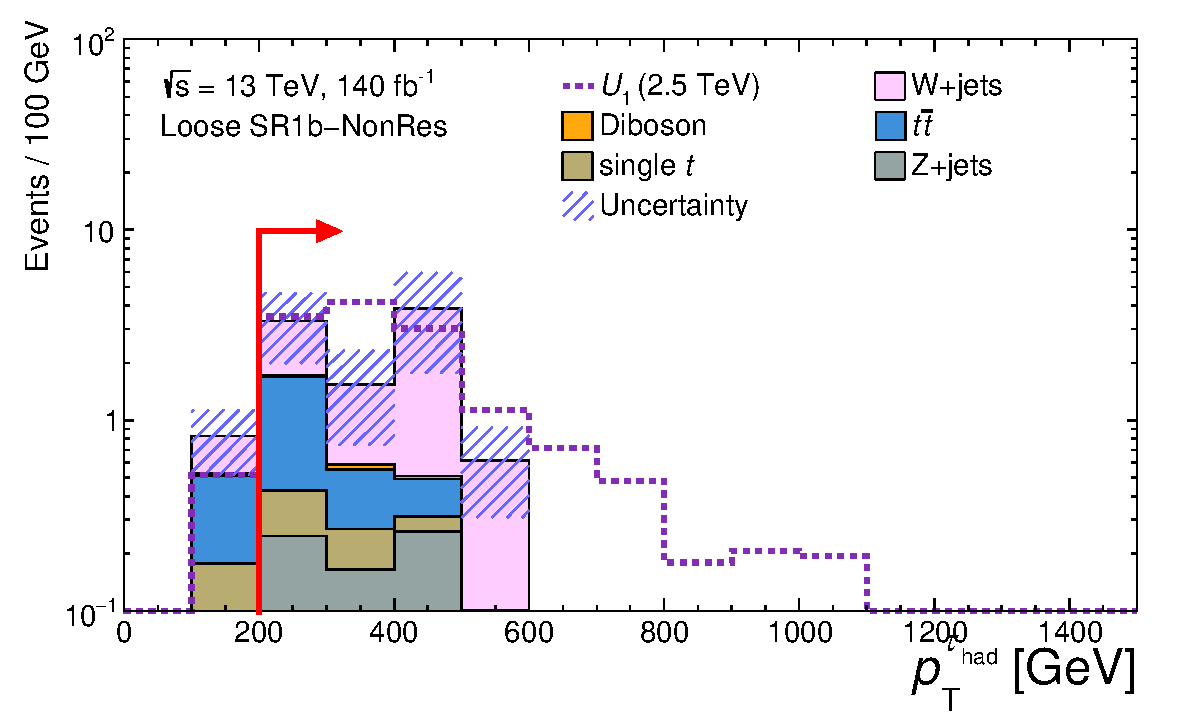
\includegraphics[width=\linewidth]{Figs/CH7/SR1b_NonRes_tau_pT.pdf}
        \caption{$\pT^{\tau_{\mathrm{had}}}$.}
    \end{subfigure}\\
    \begin{subfigure}{0.48\linewidth}
        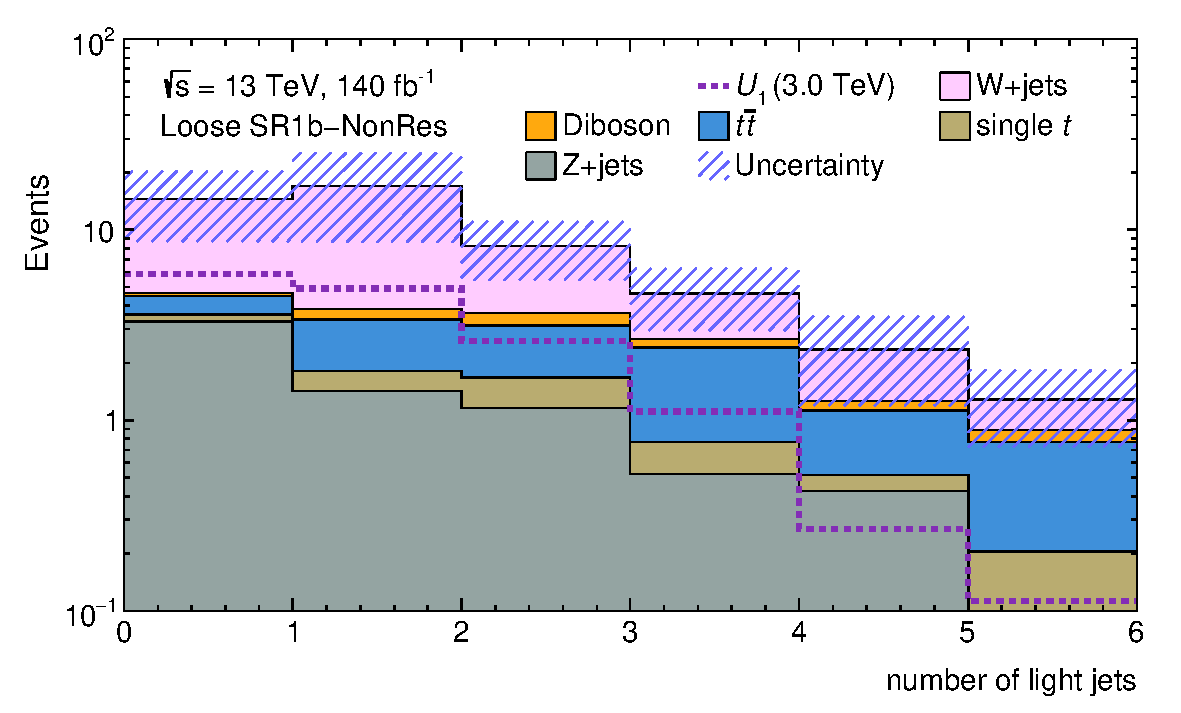
\includegraphics[width=\linewidth]{Figs/CH7/SR1b_NonRes_nlightjets.pdf}
        \caption{Number of light jets.}
    \end{subfigure}\hfill
    \begin{subfigure}{0.48\linewidth}
        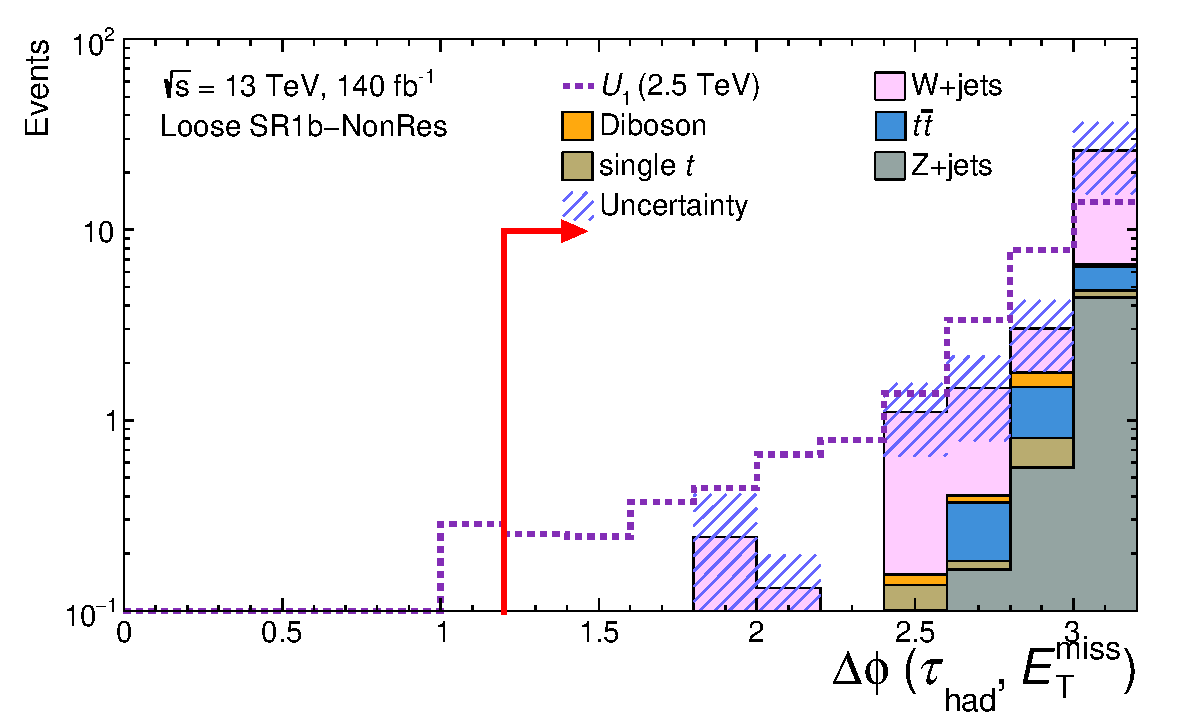
\includegraphics[width=\linewidth]{Figs/CH7/SR1b_NonRes_dphi.pdf}
        \caption{$\Delta\phi(\tau_{\mathrm{had}},\met)$.}
    \end{subfigure}
    \caption[Loose N-1 distributions in SR1b-NonRes]{$N-1$ distributions in the loose $\bTagSR$-$\NonRes$ region. The $\mT$, $\met$ and $\pT^\tau$ thresholds are reduced to $500~\GeV$, $300~\GeV$ and $100~\GeV$, respectively. The baseline $\met>200~\GeV$ is retained. The purple dashed line represents the signal at $(\MU,\gU,\beta_L^{23})=(2.5~\TeV,2.5,1.0)$. Systematic uncertainties are also included. The red arrows indicate the final selection thresholds.}
    \label{fig:ch7_sr1b_nonres_distributions}
\end{figure}

\clearpage
\section[b-veto signal region (SR0b)]{$b$-veto signal region ($\bVetoSR$)}
\label{sec:ch7_sr0b}

The $\bVetoSR$ regions are defined based on the $\bTagSR$ optimisation results, targeting on-shell $U_1\to s\tau$ decays to extend the sensitivity to large $\beta_L^{23}$.
The corresponding signal topologies were introduced in Section~\ref{subsec:lq_collider_benchmark}.
In particular, the event selection is retained except that the $b$-jet requirement is replaced by a requirement on a non-$b$-tagged jet. The $\pT^b$ requirement is applied to the leading jet instead. The final definitions of all SRs are summarised in Table~\ref{tab:ch7_signal_regions}.

\begin{table}[htbp]
    \centering
    \small
    \caption{Common baseline requirements and final signal-region selections. A dash denotes no additional requirement. The jet multiplicity includes $b$-tagged jets.}
    \label{tab:ch7_signal_regions}
    \begin{tabular}{lcccc}
        \toprule
        \multicolumn{5}{c}{Baseline requirements} \\
        \midrule
        Trigger & \multicolumn{4}{c}{Lowest-threshold unprescaled $\met$ trigger} \\
        $N_\tau$ & \multicolumn{4}{c}{1} \\
        $N_\ell=N_e+N_\mu$ & \multicolumn{4}{c}{0} \\
        Multijet suppression & \multicolumn{4}{c}{$\minDphiJetMet>0.4$ or $\metOverMinDphiJetPt>6$} \\
        \midrule
        & \multicolumn{2}{c}{Resonant} & \multicolumn{2}{c}{Non-resonant} \\
        Requirement & $\bTagSR$-$\Res$ & $\bVetoSR$-$\Res$ & $\bTagSR$-$\NonRes$ & $\bVetoSR$-$\NonRes$ \\
        \midrule
        $N_b$ & 1 & 0 & 1 & 0 \\
        $\pT^b$ [$\GeV$] & $>250$ & -- & $50<\pT^b<250$ & -- \\
        $\pT^{j_1}$ [$\GeV$] & -- & $>250$ & -- & $50<\pT^{j_1}<250$ \\
        $\pT^\tau$ [$\GeV$] & \multicolumn{4}{c}{$>200$} \\
        $\met$ [$\GeV$] & \multicolumn{2}{c}{$>200$} & \multicolumn{2}{c}{$>400$} \\
        $\mT$ [$\GeV$] & \multicolumn{2}{c}{$>200$} & \multicolumn{2}{c}{$>600$} \\
        $m_{b\tau}$ [$\GeV$] & $>800$ & -- & -- & -- \\
        $m_{j\tau}$ [$\GeV$] & -- & $>800$ & -- & -- \\
        $\DphiTauMet$ & \multicolumn{2}{c}{--} & \multicolumn{2}{c}{$>1.2$} \\
        $N_j$ & \multicolumn{2}{c}{$\leq4$} & \multicolumn{2}{c}{$\leq2$} \\
        \bottomrule
    \end{tabular}
\end{table}


The flavour of the leading jet is identified in the truth-level study using the parton label assigned to the jet (\texttt{PartonTruthLabelID}), where 3, 4 and 21 denote $s$ quarks, $c$ quarks and gluons, respectively.
The distributions at $(\MU,\gU,\beta_L^{23})=(1.5~\TeV,1.5,0.6)$ are shown in Figure~\ref{fig:ch7_sr0b_truth_jet_flavour}.
In $\bVetoSR$-$\Res$, approximately $30\%$ of the events contain a leading $s$ jet and $60\%$ contain a leading $c$ jet. The $s$-jet contribution is produced through single leptoquark production followed by $U_1\to s\tau$ decays, which are enhanced at large $\beta_L^{23}$.
For the $c$-jet contribution, a high-$\pT$ $c$ jet is produced in an on-shell $U_1\to c\nu_\tau$ decay, as illustrated in Figure~\ref{fig:ch7_sr0b_cnu_diagram}.
In $\bVetoSR$-$\NonRes$, approximately $33\%$ of the events are produced through non-resonant $\tau\nu$ production with a $c$ jet from initial-state radiation (ISR), while $11\%$ contain an ISR $s$ jet.
The remaining events are mainly produced through $sc\to\tau\nu_\tau$ with an ISR gluon jet.

\begin{figure}[htpb]
    \centering
    \begin{subfigure}{0.48\linewidth}
        \includegraphics[width=\linewidth]{Figs/CH7/truth_flavour/SR0b_Res_leading_jet_parton_ID.pdf}
        \caption{$\bVetoSR$-$\Res$.}
    \end{subfigure}\hfill
    \begin{subfigure}{0.48\linewidth}
        \includegraphics[width=\linewidth]{Figs/CH7/truth_flavour/SR0b_NonRes_leading_jet_parton_ID.pdf}
        \caption{$\bVetoSR$-$\NonRes$.}
    \end{subfigure}
    \caption[Leading-jet flavour in SR0b]{Leading-jet parton-ID distributions in $\bVetoSR$-$\Res$ and $\bVetoSR$-$\NonRes$, at the signal point $(\MU,\gU,\beta_L^{23})=(1.5~\TeV,1.5,0.6)$. The parton IDs 3, 4 and 21 denote $s$ quarks, $c$ quarks and gluons, respectively.}
    \label{fig:ch7_sr0b_truth_jet_flavour}
\end{figure}

\begin{figure}[htpb]
    \centering
    \includegraphics[width=0.32\linewidth]{Figs/CH7/truth_flavour/SR0b_Res_cnu_diagram.pdf}
    \caption[Signal diagram with a leading charm jet in SR0b-Res]{Signal diagram contributing to $\bVetoSR$-$\Res$ through an on-shell $U_1\to c\nu_\tau$ decay.}
    \label{fig:ch7_sr0b_cnu_diagram}
\end{figure}


The interference contribution in $\bVetoSR$ is evaluated at each signal parameter point.
Since it is not CKM-suppressed, a larger destructive interference contribution is expected. The total signal yield is found to be reduced by approximately $20\%$ at $\MU=1.5~\TeV$ and by about $30$--$40\%$ at higher masses. However, it remains positive over the parameter region probed by this analysis.
The supplementary $\met$ scan in Appendix~\ref{app:sr0b_optimisation} shows that a higher $\met$ threshold can suppress this contribution. This improvement can be used in the next LQ search with the full Run~3 dataset.
The $N-1$ distributions for $\bVetoSR$-$\Res$ and $\bVetoSR$-$\NonRes$ are shown in Figures~\ref{fig:ch7_sr0b_distributions} and~\ref{fig:ch7_sr0b_nonres_distributions}, respectively.

\begin{figure}[htpb]
    \centering
    \begin{subfigure}{0.48\linewidth}
        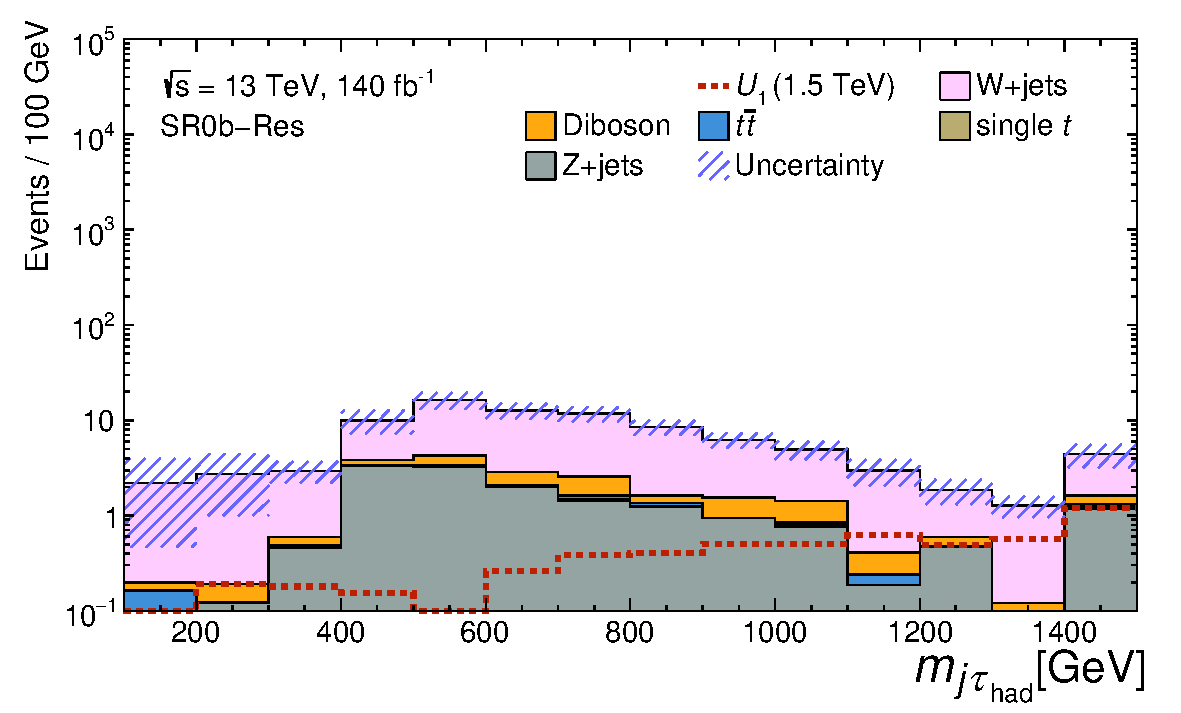
\includegraphics[width=\linewidth]{Figs/CH7/SR0b_Res_InvM.pdf}
        \caption{$m_{j\tau_{\mathrm{had}}}$.}
    \end{subfigure}\hfill
    \begin{subfigure}{0.48\linewidth}
        \includegraphics[width=\linewidth]{Figs/CH7/SR0b_Res_met.pdf}
        \caption{$\met$.}
    \end{subfigure}\\
    \begin{subfigure}{0.48\linewidth}
        \includegraphics[width=\linewidth]{Figs/CH7/SR0b_Res_mT.pdf}
        \caption{$\mT$.}
    \end{subfigure}\hfill
    \begin{subfigure}{0.48\linewidth}
        \includegraphics[width=\linewidth]{Figs/CH7/SR0b_Res_tau_pT.pdf}
        \caption{$\pT^{\tau_{\mathrm{had}}}$.}
    \end{subfigure}\\
    \begin{subfigure}{0.48\linewidth}
        \includegraphics[width=\linewidth]{Figs/CH7/SR0b_Res_njets.pdf}
        \caption{Number of jets.}
    \end{subfigure}\hfill
    \begin{subfigure}{0.48\linewidth}
        \includegraphics[width=\linewidth]{Figs/CH7/SR0b_Res_jet_pt.pdf}
        \caption{$\pT^{\mathrm{leading\ jet}}$.}
    \end{subfigure}
    \caption[N-1 distributions in SR0b-Res]{$N-1$ distributions in $\bVetoSR$-$\Res$. The baseline $\met>200~\GeV$ requirement is kept. The red dashed line represents the signal at $(\MU,\gU,\beta_L^{23})=(1.5~\TeV,1.5,0.6)$. Systematic uncertainties are also included. The red arrows indicate the final selection thresholds.}
    \label{fig:ch7_sr0b_distributions}
\end{figure}

\begin{figure}[htpb]
    \centering
    \begin{subfigure}{0.48\linewidth}
        \includegraphics[width=\linewidth]{Figs/CH7/SR0b_NonRes_met.pdf}
        \caption{$\met$.}
    \end{subfigure}\hfill
    \begin{subfigure}{0.48\linewidth}
        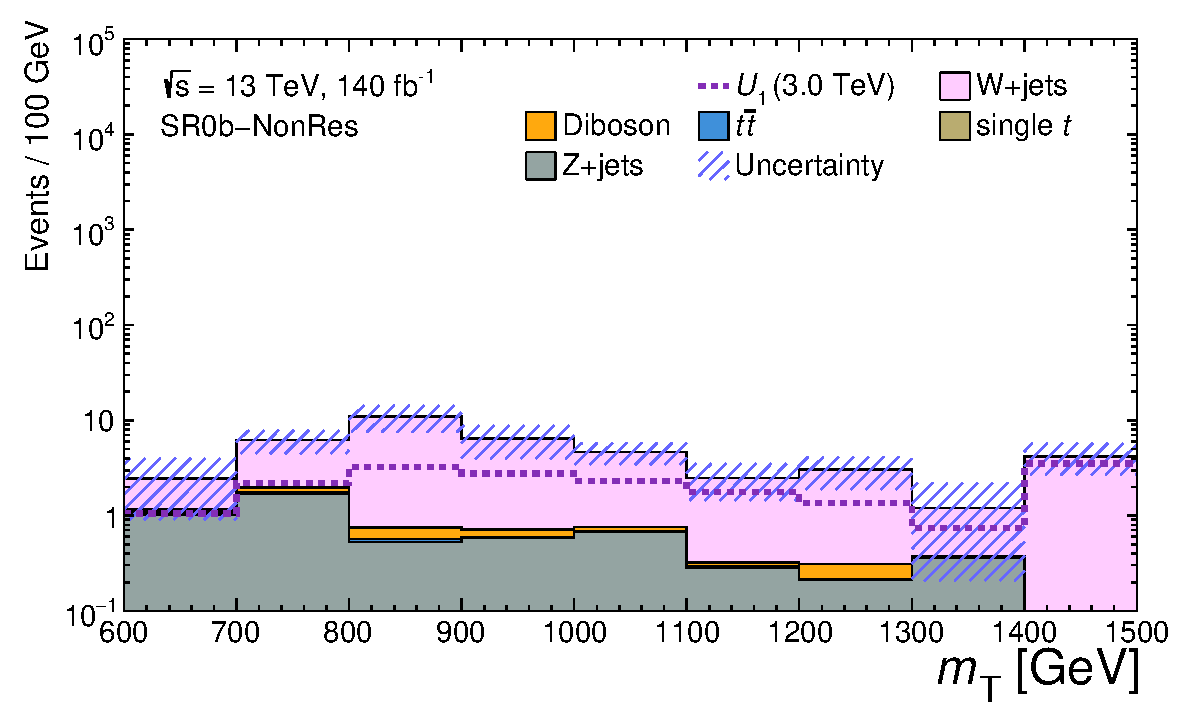
\includegraphics[width=\linewidth]{Figs/CH7/SR0b_NonRes_mT.pdf}
        \caption{$\mT$.}
    \end{subfigure}\\
    \begin{subfigure}{0.48\linewidth}
        \includegraphics[width=\linewidth]{Figs/CH7/SR0b_NonRes_tau_pT.pdf}
        \caption{$\pT^{\tau_{\mathrm{had}}}$.}
    \end{subfigure}\hfill
    \begin{subfigure}{0.48\linewidth}
        \includegraphics[width=\linewidth]{Figs/CH7/SR0b_NonRes_jet_pt.pdf}
        \caption{$\pT^{\mathrm{leading\ jet}}$.}
    \end{subfigure}\\
    \begin{subfigure}{0.48\linewidth}
        \includegraphics[width=\linewidth]{Figs/CH7/SR0b_NonRes_njets.pdf}
        \caption{Number of jets.}
    \end{subfigure}\hfill
    \begin{subfigure}{0.48\linewidth}
        \includegraphics[width=\linewidth]{Figs/CH7/SR0b_NonRes_dphi.pdf}
        \caption{$\Delta\phi(\tau_{\mathrm{had}},\met)$.}
    \end{subfigure}
    \caption[N-1 distributions in SR0b-NonRes]{$N-1$ distributions in $\bVetoSR$-$\NonRes$. The baseline $\met>200~\GeV$ requirement is kept. The purple dashed line represents the signal at $(\MU,\gU,\beta_L^{23})=(2.5~\TeV,2.5,1.0)$. Systematic uncertainties are also included. The red arrows indicate the final selection thresholds.}
    \label{fig:ch7_sr0b_nonres_distributions}
\end{figure}

The $\bVetoSR$ is dominated by $W\to\tau\nu$+jets, since vetoing $b$-jets removes much of the top-quark background while retaining $W$ production with light-flavour jets.
Specifically, $W$+jets contributes approximately $76\%$ in $\bVetoSR$-$\Res$ and $82\%$ in $\bVetoSR$-$\NonRes$.
In the resonant region, diboson production contributes about $10\%$, $Z\to\nu\nu$+jets about $8\%$, and $Z\to\tau\tau$+jets about $5\%$.
In the non-resonant region, the corresponding contributions are approximately $3\%$, $6\%$ and $8\%$.
The $Z\to\nu\nu$, $Z\to\tau\tau$ and diboson events have a similar topology to that in $\bTagSR$, while the top-quark background contribution is negligible.

\clearpage
\section{$\tau\tau$ signal contamination} \textcolor{red}{Perhaps this section should be moved to the appendix?}
\label{sec:ch7_tautau_contamination}

The signal contamination $\tau\tau$ production is evaluated in this section.
Although two $\tau$-leptons are produced in the final state, an event can satisfy the single-$\tau$ requirement when only one is reconstructed and selected. Neutrinos from the $\tau$ decays produce missing momentum.

The study uses simulated $\tau\tau$ samples generated with $\beta_L^{33}=1$, $\beta_R^{33}=0$ and $\beta_L^{23}=0$.
Their yields are compared with those of the available $\tau\nu+b$ samples near the expected exclusion limit, at $(\MU,\gU,\beta_L^{23})=(1.8~\TeV,3.0,0.6)$ and $(3.0~\TeV,2.0,1.4)$.
The corresponding $\tau\tau$ samples use $\gU=2.8$ and $2.1$.
Since the $\tau\tau$ samples are generated at $\beta_L^{23}=0$, a fair comparison with the $\tau\nu+b$ samples at the same $\beta_L^{23}$ is not directly possible. To address this, the $\tau\tau$ production cross section is recalculated with \textsc{MadGraph5\_aMC@NLO} at the corresponding $\beta_L^{23}$, and the yields of the $\tau\tau$ samples at $\beta_L^{23}=0$ are corrected by the cross-section ratios to $\beta_L^{23}=0.6$ and $1.4$. Specifically, the cross-section ratios are $\sigma_{\beta_L^{23}=0.6}/\sigma_{\beta_L^{23}=0}=2.7$ and $\sigma_{\beta_L^{23}=1.4}/\sigma_{\beta_L^{23}=0}=30$.
This procedure therefore provides a sensitivity study while retaining the acceptance and kinematic shapes of the available samples. For simplicity, the signal theory uncertainty is not included in this study.

The $\tau\nu$ yields and estimated $\tau\tau$ contributions are summarised in Table~\ref{tab:ch7_tautau_contamination}.
The estimated contamination from $\tau\tau$ production is of order $35\%$ of the nominal $\tau\nu$ yield in $\bTagSR$, and several percent in $\bVetoSR$.

\begin{table}[htbp]
    \centering
    \small
    \setlength{\tabcolsep}{3pt}
    \caption[Signal yields from $\tau\nu$ and $\tau\tau$ production in the SRs]{Signal yields from $\tau\nu$ and $\tau\tau$ production in the four SRs. The parameter values $(\MU,\gU,\beta_L^{23})$ are given for each sample. The $\tau\tau$ yields are shown at $\beta_L^{23}=0$, with the yields scaled to $\beta_L^{23}=0.6$ and $1.4$, respectively, given in parentheses.}
    \label{tab:ch7_tautau_contamination}
    \begin{tabular}{lcccc}
        \toprule
        Region & $\tau\nu$ & $\tau\nu$ & $\tau\tau$ & $\tau\tau$ \\
        & $(1.8~\TeV,3.0,0.6)$ & $(3.0~\TeV,2.0,1.4)$ & $(1.8~\TeV,2.8,0)$ & $(3.0~\TeV,2.1,0)$ \\
        \midrule
        $\bTagSR$-$\Res$ & 21.0 & 2.2 & 2.5 (6.75) & 0.03 (0.9) \\
        $\bTagSR$-$\NonRes$ & 11.8 & 3.3 & 1.3 (3.51) & 0.04 (1.2) \\
        $\bVetoSR$-$\Res$ & 28.9 & 7.5 & 0.8 (2.16) & 0.01 (0.3) \\
        $\bVetoSR$-$\NonRes$ & 43.5 & 21.4 & 1.3 (3.51) & 0.04 (1.2) \\
        \bottomrule
    \end{tabular}
\end{table}

In the further study, the expected exclusion limit on the signal strength is improved by approximately $8$--$14\%$, depending on $\MU$. Since the signal strength scales as $\gU^4$ and $(\beta_L^{23})^2$, the improvement in the coupling limit is much less significant. The expected improvement is about $5\%$ at $\MU=1.8~\TeV$ and about $2\%$ at $\MU=3.0~\TeV$.
Therefore, the sensitivity is slightly underestimated if the contamination from $\tau\tau$ production is not included, but the improvement in the coupling limit is not significant and is mostly covered by the signal theory uncertainties.
